\chapter{Clang Analysis}

\section{Introduction}

In this chapter it will be described the analysis process for all the tools used.\newline\newline
\textbf{Understand} is indeed the tools that gives the most accurate results in terms of checks, since it incorporates C/C++ MISRA standards, a beta version of the \textbf{CLang Static Analyzer}, which is a static analysis tool provided by the LLVM developers, and many other quality checks offered by SciTools itself.\newline
A simpler but also quite effective tool is \textbf{Cppcheck} which is designed to "provide unique code analysis to detect bugs and to focus on detecting undefined behaviour and dangerous coding constructs" \cite{bibitem2}. Also, as pointed by the developers, its main focus is to  "detect only real errors in the code (i.e. have very few false positives)". Cppcheck refers to the \textsl{Common Weakness Enumeration} standard for the analysis, a formal list of security issues published by the MITRE institute. It is also possible to check MISRA-C project compliance but it requires to buy the standard so this feature was not used. \newline
The last used tool is \textbf{flawfinder} which puts its focus more on security flaws rather than quality issues. This tool incorporates an option to run the analysis in order to detect possible false positives in an automated manner. This tools uses the CWE standard as Cppcheck does.\newline
Other tools such as \textbf{SonarQube} and \textbf{Cert C Rosechecker} were used but due to their characteristics they were unusable for our purpose.
\pagebreak

\section{Analysis Methodology}

The LLVM Clang compiler was analized with all the tools listed above.\newline
Since some issues arose while analyzing the whole project, as it was pointed in the previous section, a representative subset of it was chosen. In particular the folder \textbf{src/tool/libclang} was analyzed because it has been observed that the source files in this folder contained much of the compiler logic. This was the input folder for all the static analysis tools used.\newline\newline
After the output was produced, the second phase of the analysis can start. Since the output format of the various tool is hetherogenous, it was necessary to convert them in excel sheets in order to collect evidences about what files were the most vulnerable/contained more bugs.

\section{Understand}

Understand is a very powerful tool for static analysis that can be used to analyze software written in multiple languages suchs as Java, Ada, Cobol, Python, C/C++\dots
Among the tools used, it is the only one that comes with a nice and user-friendly user interface that allows users to navigate through the software files.

\subsection{Understand Project}

First of all, it must be created an \textsl{Understand Project}. In this first step you are asked to select the language of the software (C/C++ in our case study) and the directories to analyze.\newline\newline
\vspace{1cm}
\begin{minipage}{\linewidth}
	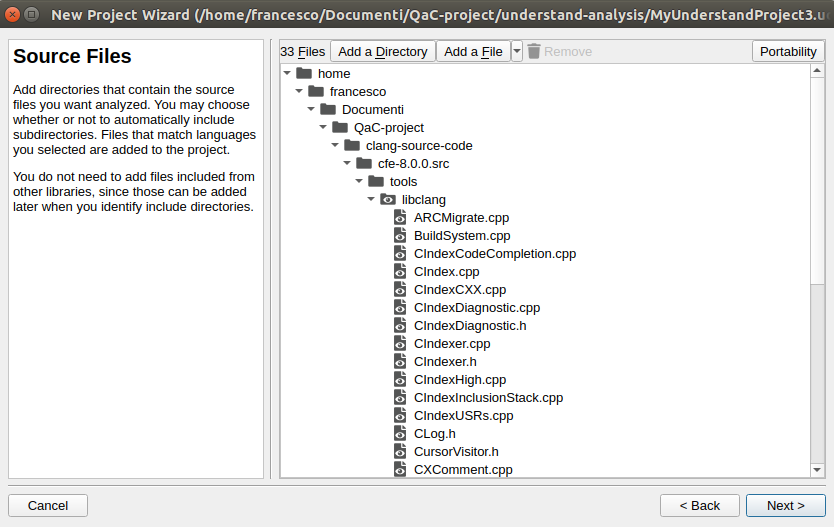
\includegraphics[width=\textwidth]{img/libclangDirectory.png}
	\captionof{figure}{The whole subdirectory tools/libclang is imported in the Understand project in order to run the analysis.}
\end{minipage}

When the files are loaded in the program, the analysis can be run simply by opening the \textsl{codecheck perspective} and selecting which standard should guide it.\newline\newline
\vspace{1cm}
\begin{minipage}{\linewidth}
	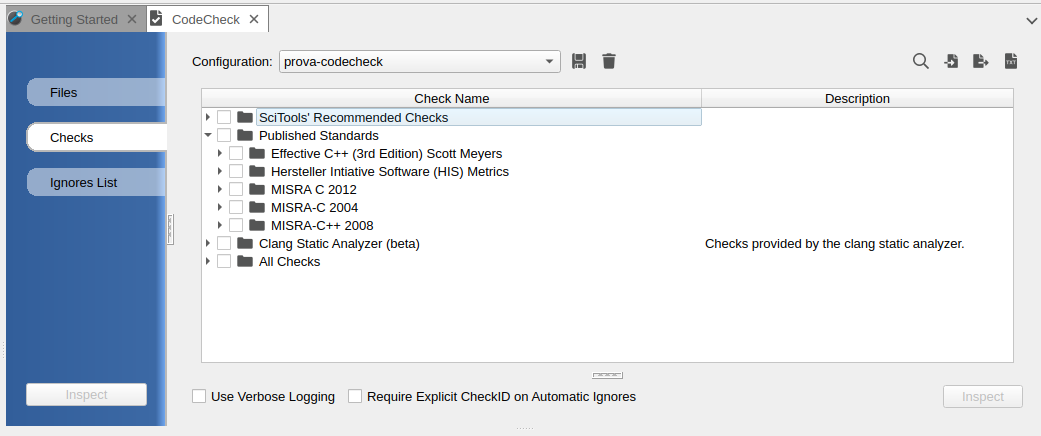
\includegraphics[width=\textwidth]{img/Codecheck.png}
	\captionof{figure}{The MISRA standard is incorporated in Understand, as well as the Clang Static Analyzer. Generic checks are also offered by the tool as \textsl{SciTools Recommended Checks} and \textsl{AllChecks}, some of which are redundant.}
\end{minipage}

\begin{itemize}
	\item \textsl{SciTools' Recommended Checks} - This is a small set (17 items) of generic good programming rules
	\item \textsl{Published Standards} - This section contains the published standards supported by Understand
		\begin{itemize}
			\item It was used the MISRA-C++ 2008 due to the nature of the source files (.cpp) and because one of the goals of this project was to check the Clang compiler compliance to MISRA rules.
		\end{itemize}
	\item \textsl{Clang Static Analyzer} - Is an implementation of the tool incorporated in Understand.
	\item \textsl{All Checks} - This is a collection of checks which consists of generic good programming rules and some of the MISRA rules. Despite its name, not all the checks are included for real, this is the reason why it is not correct to use only this option for a consistent analysis.
\end{itemize}

\subsection{Understand Output Format}

When the analysis ends, it is possible to navigate through different perspectives of what has been observed. For example it is possible to list results \textsl{by file}, in order to check which issues are present in each file (and at which line of code) and what files contains the most issues. Another possibility is to display result \textsl{by check}, that is: for each rule (e.g. MISRA) how many times it has been violated and where (in terms of files).\newline
Two very interesting features offered by Understand are the:
\begin{itemize}
	\item Result Locator
	\item Result Treemap
\end{itemize}

The first one offers the possibility to navigate through the findings, filtering them by file, by violation and some other options, giving the possibility to jump to the desired \textsl{vulnerable} line of code in the source file.\newline
The result treemap instead gives you a graphic representation of the files vulnerabilities, in terms of criticity and quantity. These characteristics can be viewed graphically using colored boxes, where the meaning of the color/dimension of the boxes can be defined by the user.\newline
Mastering the options of these two powerful features gives to the user much more control of the analysis and a wider perspective of the whole project quality.\newline\newline

\vspace{1cm}
\begin{minipage}{\linewidth}
	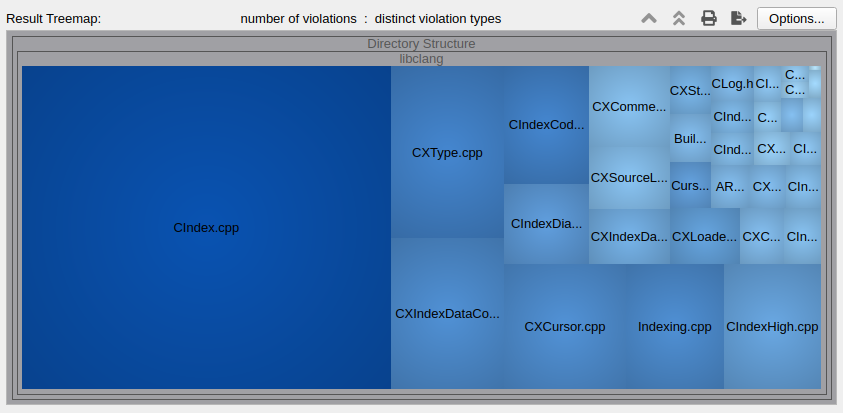
\includegraphics[width=\textwidth]{img/AllChecksTreeMap.png}
	\captionof{figure}{Result Treemap view.}
\end{minipage}
\vspace{1cm}

All the output perspectives can be exported in suitable formats (e.g. Treemap is exported in .png files while lists of violations are exported in .txt or .html files) that facilitate the second phase of the analysis.

\subsection{Understand Results}

As it has been said in the introduction, multiple analysis with different checks were ran:
\begin{itemize}
	\item[$a)$] MISRA-C++ 2008
	\item[$b)$] SciTools' Recommended Checks
	\item[$c)$] Clang Static Analyzer
	\item[$d)$] All Checks
\end{itemize}

\hspace{-0.6cm} $a)$  
This check is based on the MISRA-C++ 2008 standard, which is a standard developed for the quality of C++ source files.\newline
Results has been sorted by files and by MISRA rules. After that a compact view of these was produced showing the numbers of violations for each MISRA and for each file.\newline
Analyzing the reports it can be observed that:
\begin{itemize}
	\item The total number of violations in the \textbf{libclang} folder is 8450
	\item The first three rules that were violated the most are:
	\begin{itemize}
		\item[$1.\:$] MISRA08\_7-1-1 - \textbf{A variable which is not modified shall be const qualified} - 1845 violations.\newline If a variable does not need to be modified, then it shall be declared with const qualification so that it cannot be modified. A non-parametric variable will then require its initialization at the point of declaration. Also, future maintenance cannot accidentally modify the value.
		\item[$2.\:$] MISRA08\_6-4-1 - \textbf{An if condition construct shall be followed by a compund statement. The else keyword shall be followed by either a compound statement or another if statement} - 1239 violations.\newline If the bodies of these constructs are not compound statements, then errors can occur if a developer fails to add the required braces when attempting to change a single statement body to a multistatement body.
		Requiring that the body of these constructs shall be a compound statement (enclosed within braces) ensures that these errors cannot arise.
		\item[$3.\:$] MISRA08\_0-1-10 -\textbf{All defined functions called} - 733 violations.\newline Functions or procedures that are not called may be symptomatic of a serious problem, such as missing paths.
	\end{itemize}
	\item The first three files that contains the most violations are:
		\begin{itemize}
		\item[$1.\:$] CIndex.cpp - 3828 violations.
		\item[$2.\:$] CXType.cpp - 757 violations.
		\item[$3.\:$] CXCursor.cpp - 558 violations.
	\end{itemize}
\end{itemize}


\begin{minipage}{\linewidth}
	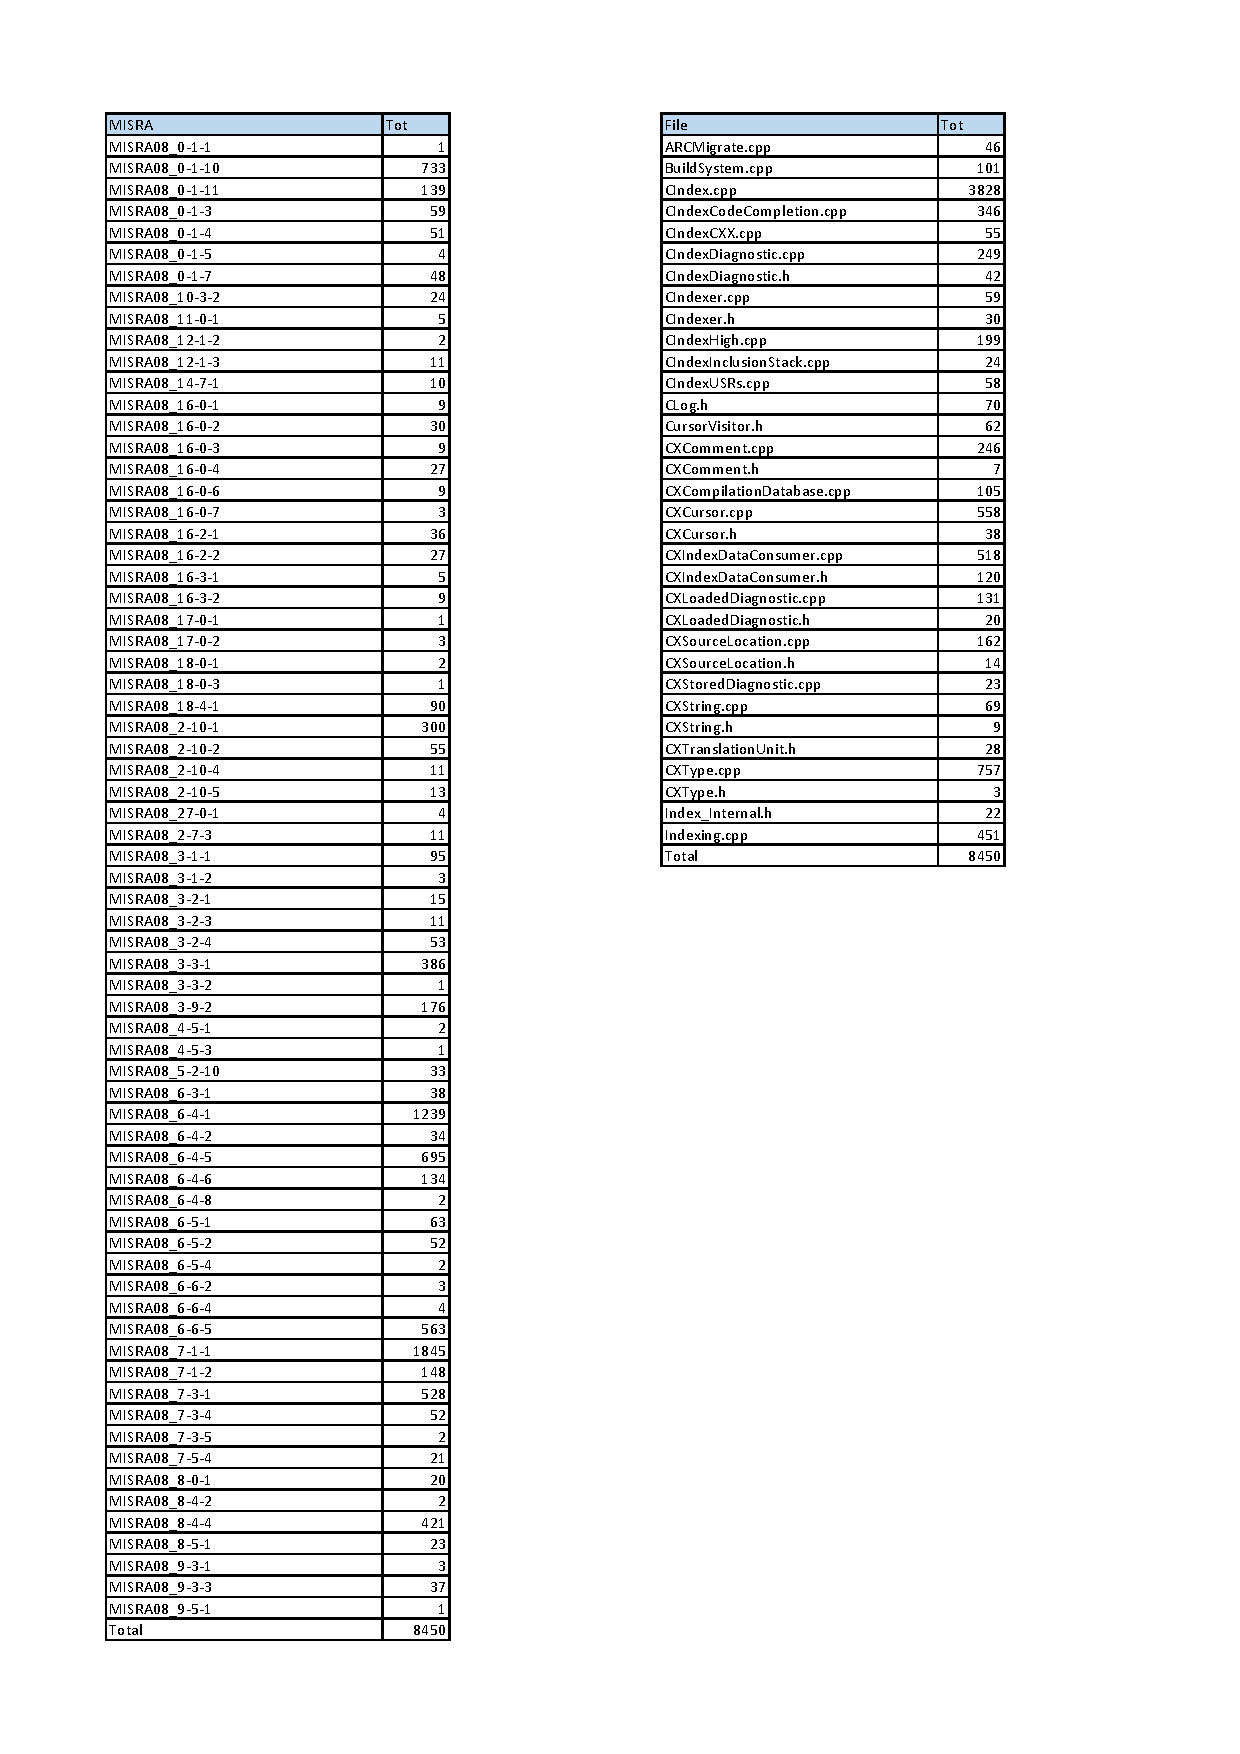
\includegraphics[width=\textwidth]{pdf/Misra_Summary.pdf}
	\captionof{figure}{Summary of the MISRA checks}
\end{minipage}

\subsection{Understand Performances}